\documentclass[12pt]{exam}
\usepackage[utf8]{inputenc}

\usepackage{amsmath,amstext,amsthm,amssymb,amsxtra}
\usepackage[top=1.5in, bottom=1.5in, left=1.25in, right=1.25in]	{geometry}
%\usepackage[normalem]{ulem}
\usepackage{txfonts} % pxfonts txfonts 
\usepackage[T1]{fontenc}
\usepackage{lmodern}
\renewcommand*\familydefault{\sfdefault}
 \usepackage{euler}   % better than the option below
\usepackage{pdfsync}
\usepackage{multicol}
\newcommand{\ci}[1]{_{ {}_{\scriptstyle #1}}}
\usepackage{graphicx}
\graphicspath{ {images/} }
\usepackage{tikz} % for drawing diagrams

\newcommand{\norm}[1]{\ensuremath{\left\|#1\right\|}}
\newcommand{\abs}[1]{\ensuremath{\left\vert#1\right\vert}}
\newcommand{\ip}[2]{\ensuremath{\left\langle#1,#2\right\rangle}}
\newcommand{\p}{\ensuremath{\partial}}
\newcommand{\pr}{\mathcal{P}}

\newcommand{\pbar}{\ensuremath{\bar{\partial}}}
\newcommand{\db}{\overline\partial}
\newcommand{\D}{\mathbb{D}}
\newcommand{\B}{\mathbb{B}}
\newcommand{\Sp}{\mathbb{S}}
\newcommand{\T}{\mathbb{T}}
\newcommand{\R}{\mathbb{R}}
\newcommand{\Z}{\mathbb{Z}}
\newcommand{\C}{\mathbb{C}}
\newcommand{\N}{\mathbb{N}}
\newcommand{\Q}{\mathbb{Q}}
\newcommand{\mQ}{\mathcal{Q}}
\newcommand{\mS}{\mathcal{S}}
\newcommand{\scrH}{\mathcal{H}}
\newcommand{\scrL}{\mathcal{L}}
\newcommand{\td}{\widetilde\Delta}
\newcommand{\pw}{\text{PW}}
\newcommand{\esup}{\text{ess.sup}}
\newcommand{\Tn}{\mathcal{T}_n}
\newcommand{\Bn}{\mathbb{B}_n}
\newcommand{\rt}{\mathcal{O}}
\newcommand{\avg}[1]{\langle #1 \rangle}
\newcommand{\one}{\mathbbm{1}}
\newcommand{\eps}{\varepsilon}
\newcommand{\grad}{\nabla}

\newcommand{\La}{\langle }
\newcommand{\Ra}{\rangle }
\newcommand{\rk}{\operatorname{rk}}
\newcommand{\card}{\operatorname{card}}
\newcommand{\ran}{\operatorname{Ran}}
\newcommand{\osc}{\operatorname{OSC}}
\newcommand{\im}{\operatorname{Im}}
\newcommand{\re}{\operatorname{Re}}
\newcommand{\tr}{\operatorname{tr}}
\newcommand{\vf}{\varphi}
\newcommand{\f}[2]{\ensuremath{\frac{#1}{#2}}}

\newcommand{\kzp}{k_z^{(p,\alpha)}}
\newcommand{\klp}{k_{\lambda_i}^{(p,\alpha)}}
\newcommand{\TTp}{\mathcal{T}_p}
\newcommand{\m}[1]{\mathcal{#1}}
\newcommand{\md}{\mathcal{D}}
\newcommand{\qan}{\abs{Q}^{\alpha/n}}
\newcommand{\sbump}[2]{[[ #1,#2 ]]}
\newcommand{\mbump}[2]{\lceil #1,#2 \rceil}
\newcommand{\cbump}[2]{\lfloor #1,#2 \rfloor}

\newcommand{\class}{Math 629 Spring 26}
\newcommand{\term}{Fall 24}
\newcommand{\examnum}{Homework \hwnum}
\newcommand{\examdate}{\duedate}
\newcommand{\timelimit}{75 Minutes}
\newcommand{\vc}[3]{\langle #1,#2,#3\rangle}
\newcommand*{\vv}[1]{\vec{\mkern0mu#1}}
\newcommand{\bv}[1]{\boldsymbol{#1}}
\newcommand{\hide}[1]{}
\newcommand{\uvec}[1]{\boldsymbol{\hat{\textbf{#1}}}}
\newcommand{\vex}[1]{\boldsymbol{{\textbf{#1}}}}

\pagestyle{head}
\firstpageheader{}{}{}
\runningheader{\class}{\examnum\ - Page \thepage\ of \numpages}{\examdate}
\runningheadrule

\makeatletter
\renewcommand*\env@matrix[1][*\c@MaxMatrixCols c]{%
  \hskip -\arraycolsep
  \let\@ifnextchar\new@ifnextchar
  \array{#1}}
\makeatother

%\printanswers
\begin{document}

\noindent
\begin{tabular*}{\textwidth}{l @{\extracolsep{\fill}} r @{\extracolsep{6pt}} l}
\textbf{\class} & \textbf{Name: Mengxiang Jiang}\\
\end{tabular*}\\
\rule[2ex]{\textwidth}{2pt}
%

 

\newcommand{\duedate}{01/26/2026 at 11:59pm}
\newcommand\hwnum{2}

Turn this assginment in on gradescope. All work must be neat and legible. Turn in 
a ``final draft''. There should be nothing scratched out and your work should flow
generally from left to right and top to bottom. 

\begin{questions}
\question
Represent $8/9$ as a sum of fractions using Greek Notation (you can use "our" alphabet if you want). 
\\\\
Since the Greeks used unit fractions like the Egyptians, we start with:
\begin{align*}
  \frac{8}{9} &= \frac{1}{2} + \frac{7}{18} \\
  &= \frac{1}{2} + \frac{1}{3} + \frac{1}{18} \\
\end{align*}
Using the notation listed in the book, we have:
\[
  \angle \acute \gamma \acute \iota \acute \eta
\]
\newpage
\question 
Show that the $N$th triangular number is $\frac{N(N+1)}{2}$ and thus an oblong number is double a triangular number. 
\\\\
The $N$th triangular number is the sum of the first $N$ natural numbers:
\[
  T_N = 1 + 2 + 3 + \dots + N
\]
Since this is a finite sum, we can apply the commutative property of addition and rearrange the terms:
\[
  T_N = N + (N-1) + (N-2) + \dots + 1
\]
Adding the two expressions for $T_N$ together, we get:
\begin{align*}
  2T_N &= (1+N) + (2+(N-1)) + (3+(N-2)) + \dots + (N+1) \\
        &= (N+1) + (N+1) + (N+1) + \dots + (N+1) \\
        &= N(N+1)
\end{align*}
Since this is double the triangular number, we divide both sides by 2 to get:
\[
  T_N = \frac{N(N+1)}{2}
\]
\newpage 
\question 
Using dots/pebbles, show that eight times any triangular number plus 1 makes a square. 
\\\\
Since the $N$th triangular number is $\frac{N(N+1)}{2}$, eight times the $N$th triangular number plus 1 is:
\[
  8 \cdot \frac{N(N+1)}{2} + 1 = 4N(N+1) + 1 = 4N^2 + 4N + 1 = (2N + 1)^2
\]
Thus, I know that the square I need to draw will have side length $2N + 1$. Here is the diagram for $N=4$:
\begin{center}
  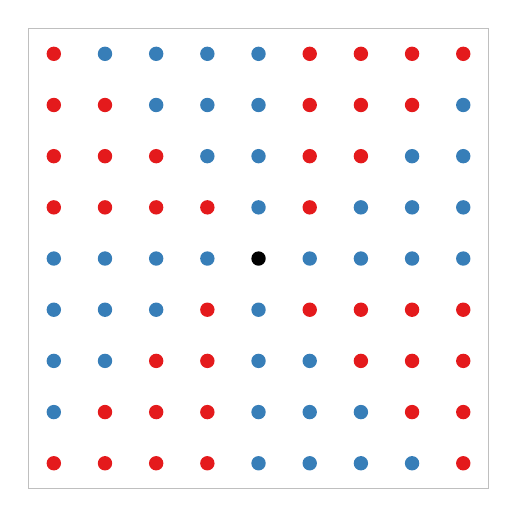
\begin{tikzpicture}[scale=0.65]

  % Two colors only (checkerboard across the 8 triangles)
  \definecolor{cA}{RGB}{55,126,184}   % blue
  \definecolor{cB}{RGB}{228,26,28}    % red
  \def\r{4pt}

  % Outline of the (2N+1)x(2N+1) dot-square, here 9x9 (since N=4)
  \draw[black!25] (-4.5,-4.5) rectangle (4.5,4.5);

  % ---- 8 triangles, each has T_4=10 dots. Adjacent triangles alternate colors ----
  % Triangle 1 (E axis) - cA
  \foreach \x/\y in {1/0,2/0,2/1,3/0,3/1,3/2,4/0,4/1,4/2,4/3}
    \fill[cA] (\x,\y) circle (\r);

  % Triangle 2 (NE diagonal) - cB
  \foreach \x/\y in {1/1,1/2,1/3,1/4,2/2,2/3,2/4,3/3,3/4,4/4}
    \fill[cB] (\x,\y) circle (\r);

  % Triangle 3 (N axis) - cA
  \foreach \x/\y in {-3/4,-2/3,-2/4,-1/2,-1/3,-1/4,0/1,0/2,0/3,0/4}
    \fill[cA] (\x,\y) circle (\r);

  % Triangle 4 (NW diagonal) - cB
  \foreach \x/\y in {-4/1,-4/2,-4/3,-4/4,-3/1,-3/2,-3/3,-2/1,-2/2,-1/1}
    \fill[cB] (\x,\y) circle (\r);

  % Triangle 5 (W axis) - cA
  \foreach \x/\y in {-4/-3,-4/-2,-4/-1,-4/0,-3/-2,-3/-1,-3/0,-2/-1,-2/0,-1/0}
    \fill[cA] (\x,\y) circle (\r);

  % Triangle 6 (SW diagonal) - cB
  \foreach \x/\y in {-4/-4,-3/-4,-3/-3,-2/-4,-2/-3,-2/-2,-1/-4,-1/-3,-1/-2,-1/-1}
    \fill[cB] (\x,\y) circle (\r);

  % Triangle 7 (S axis) - cA
  \foreach \x/\y in {0/-4,0/-3,0/-2,0/-1,1/-4,1/-3,1/-2,2/-4,2/-3,3/-4}
    \fill[cA] (\x,\y) circle (\r);

  % Triangle 8 (SE diagonal) - cB
  \foreach \x/\y in {1/-1,2/-2,2/-1,3/-3,3/-2,3/-1,4/-4,4/-3,4/-2,4/-1}
    \fill[cB] (\x,\y) circle (\r);

  % The "+1" center dot
  \fill[black] (0,0) circle (\r);

  \end{tikzpicture}
\end{center}



\newpage 
\question 
Show that in a Pythagorean triple, if one of the terms is odd, then two of them must be odd and one even. 
\\\\
Let the Pythagorean triple be $(a,b,c)$ such that $a^2 + b^2 = c^2$. We will consider the parity of $a$, $b$, and $c$. Assume that one of the terms is odd. We will analyze the possible cases:
\begin{itemize}
  \item Case 1: $a$ is odd.
    \begin{itemize}
      \item If $b$ is odd, then $a^2 + b^2$ is even (since odd + odd = even), making $c^2$ even, and thus $c$ is even.
      \item If $b$ is even, then $a^2 + b^2$ is odd (since odd + even = odd), making $c^2$ odd, and thus $c$ is odd.
    \end{itemize}
  \item Case 2: $b$ is odd.
    \begin{itemize}
      \item If $a$ is odd, then as in Case 1, $c$ is even.
      \item If $a$ is even, then as in Case 1, $c$ is odd.
    \end{itemize}
  \item Case 3: $c$ is odd.
    \begin{itemize}
      \item If both $a$ and $b$ are even, then $a^2 + b^2$ is even, making $c^2$ even, contradicting the assumption that $c$ is odd.
      \item If one of $a$ or $b$ is odd, this forces the other to be even (since odd + even = odd).
    \end{itemize}
\end{itemize}
From the above cases, we see that if one of the terms in a Pythagorean triple is odd, then two of them must be odd and one must be even.

\end{questions}
\end{document}
